\documentclass[conference]{IEEEtran}

\usepackage{kotex}
\usepackage{amsmath,amssymb}
\usepackage{graphicx}
\usepackage{booktabs}
\usepackage{array}
\usepackage{cite}
\usepackage{url}
\usepackage{xcolor}
\usepackage{enumitem}

\graphicspath{{figures/}}
\setlength{\textfloatsep}{8pt plus 2pt minus 2pt}
\setlength{\floatsep}{8pt plus 2pt minus 2pt}
\setlength{\intextsep}{8pt plus 2pt minus 2pt}

\newcommand{\ZoneErr}{\mathrm{ZoneErr}}
\newcommand{\argmaxop}{\operatorname*{arg\,max}}
\newcommand{\argminop}{\operatorname*{arg\,min}}

\begin{document}

\title{IBR 기인 진동 배경 하에서 고장 검출 및 Zone Localization을 위한 Two-Stage Hard-Constrained WMU Placement}

\author{%
\IEEEauthorblockN{Hjin}
\IEEEauthorblockA{Department of Electrical and Electronic Engineering\\
Hanyang University\\
Email: 271123352+hjinyy@users.noreply.github.com}
}

\maketitle

\begin{abstract}
Inverter-based resource(IBR)의 비중이 증가함에 따라 전력계통 waveform에는 고장 검출을 어렵게 만드는 진동성 배경 성분이 나타날 수 있다. 동시에 load switching과 같은 비고장 switching event는 보호 관점의 고장 판단을 유발하지 않아야 한다. 본 논문은 fault detection과 fault-zone localization을 분리하는 two-stage waveform measurement unit(WMU) placement framework를 제안한다. Stage 1은 hard-constrained detection anchor WMU를 사용하며, normal false positive, LoadSwitch false positive, single-line-to-ground fault false negative, three-phase fault false negative가 모두 0이 되도록 요구한다. Stage 2는 fault decision 이후에만 활성화되며, 물리적으로 해석 가능한 current-disturbance argmax rule을 이용하여 고장을 사전 정의된 topology zone으로 localize한다. 평가는 IBR-like 25 Hz subsynchronous oscillation background, normal case, 5\%, 15\%, 30\% LoadSwitch case, SLG/three-phase fault case를 포함하는 modified IEEE 30-bus deterministic waveform dataset을 사용한다. Detection stage는 Bus 27을 one-WMU anchor로 선택하며, 평가 case에서 zero detection error와 fault-score margin 0.511616을 달성한다. Localization을 위한 exhaustive subset search 결과, $k\leq 7$ WMU subset에서는 zero zone error가 불가능하고, $k=8$에서 다섯 개의 zero-error subset이 존재함을 확인하였다. 최종 localization placement는 $\{2,11,13,16,20,23,24,27\}$이며, 이 set은 Bus 27 detection anchor를 포함하고 60개의 evaluated fault case 전체에서 zero zone-localization error를 달성한다.
\end{abstract}

\begin{IEEEkeywords}
Waveform measurement unit, WMU placement, inverter-based resources, subsynchronous oscillation, load switching, fault detection, zone localization, hard constraint, IEEE 30-bus system.
\end{IEEEkeywords}

\section{서론}

동기발전기 중심의 전력계통이 inverter-based resource(IBR) 중심의 계통으로 전환되면서 새로운 monitoring 및 protection 문제가 제기되고 있다. 기존 회전기와 달리 IBR은 converter control과 synchronization loop를 통해 계통과 상호작용한다. 이 상호작용은 converter control dynamics, network impedance, operating condition이 불리하게 결합될 때 weak grid에서 oscillatory behavior를 유발할 수 있다. Weak-grid IBR 및 wind-energy converter에 관한 선행연구들은 subsynchronous oscillation(SSO), subsynchronous control interaction, impedance-driven stability 현상을 보고하였다~\cite{liu2017subsynchronous,yuan2020investigating,liu2017mechanism,liu2019frequency,sun2011impedance,wen2016impedance,chowdhury2017nonlinear,shair2022adaptive,azimi2022supplementary,yoon2024deep}. 이러한 연구는 향후 fault monitoring이 clean pre-event waveform을 가정해서는 안 된다는 점을 시사한다.

Waveform measurement unit(WMU)은 synchronized high-resolution voltage/current waveform을 제공한다. Conventional phasor measurement unit(PMU)과 비교할 때, WMU는 transient shape, time-domain change, spectral component, phase-dependent waveform signature를 보존할 수 있다. 최근 synchro-waveform 연구들은 waveform data를 transient event localization, incipient fault detection, power-quality event classification, fault location/type identification에 활용하였다~\cite{izadi2021synchronous,izadi2022synchronized,mansourlakouraj2023waveform}. 그러나 모든 bus에 WMU를 설치하는 것이 경제적이지 않다면 placement problem이 핵심 문제가 된다.

Classical PMU placement 연구들은 complete 또는 partial network observability를 만족하면서 sensor count를 최소화하는 문제를 주로 다루었다~\cite{nuqui2005phasor,gou2008generalized,peng2006optimal,rakpenthai2007optimal,carvalho2018observability}. Fault-aware PMU placement는 이 관점을 fault observability 및 fault location으로 확장하였다~\cite{eissa2018hierarchical,pokharel2009optimal}. 이러한 formulation은 measurement placement의 중요한 기반을 제공하지만, conventional observability formulation만으로는 IBR-like oscillatory background 하에서 fault와 non-fault switching event를 waveform feature 기반으로 구별하는 제약을 직접 강제하기 어렵다.

이 구분은 중요하다. Load switching, capacitor switching, transformer energization 등은 protection 및 transient classification 문헌에서 non-fault disturbance로 다루어지는 경우가 많다~\cite{faiz2007adaptive,wang2003classification,shahrtash2006high,perera2008power,costa2010detection,hajibandeh2017classifications,sadeghkhani2016transient,bera2021discrimination,veerasamy2021lstm,zanjani2013high}. 평균 classification accuracy가 높더라도, non-fault switching event를 fault로 오분류하는 placement는 보호 관점에서 부적합할 수 있다. 따라서 본 논문은 LoadSwitch case를 non-fault event로 취급하고 zero-LoadSwitch-false-positive constraint를 명시적으로 부과한다.

본 연구의 목적은 IBR-like SSO background condition 하에서 (i) normal 및 LoadSwitch event와 fault event를 구별하고, (ii) 검출된 fault를 predefined topology zone으로 localize하는 minimum WMU placement architecture를 결정하는 것이다. 제안 결과는 지정된 feature set, topology-zone definition, decision rule 하에서의 deterministic in-dataset case-study result로 해석해야 하며, 모든 운전 조건에 대해 deployment-ready universal optimum을 주장하는 것은 아니다.

본 논문의 주요 contribution은 다음과 같다.
\begin{enumerate}[leftmargin=*]
\item Fault detection과 zone localization을 분리하는 two-stage WMU placement framework를 정식화한다.
\item Detection stage는 NormalFP=0, LoadSwitchFP=0, SLGFN=0, ThreePhaseFN=0이라는 protection-oriented hard constraints를 부과한다.
\item Localization stage는 installed WMU set에 대해 물리적으로 해석 가능한 $dI\_energy_{3ph,max}$ argmax rule을 사용한다.
\item Exhaustive subset search를 통해 지정된 formulation 하에서 첫 번째 zero-zone-error localization solution이 $k=8$에서 나타남을 보인다.
\item 최종 installed set $\{2,11,13,16,20,23,24,27\}$은 localization constraint를 만족하면서 Bus 27 detection anchor를 포함한다.
\end{enumerate}

\section{제안하는 Two-Stage Framework}

Fig.~\ref{fig:framework}는 제안하는 two-stage framework를 요약한다. 첫 번째 stage는 event가 fault인지 non-fault인지 판별한다. 두 번째 stage는 fault로 검출된 case에 대해서만 활성화되며, faulted topology zone을 추정한다.

\begin{figure*}[t]
\centering
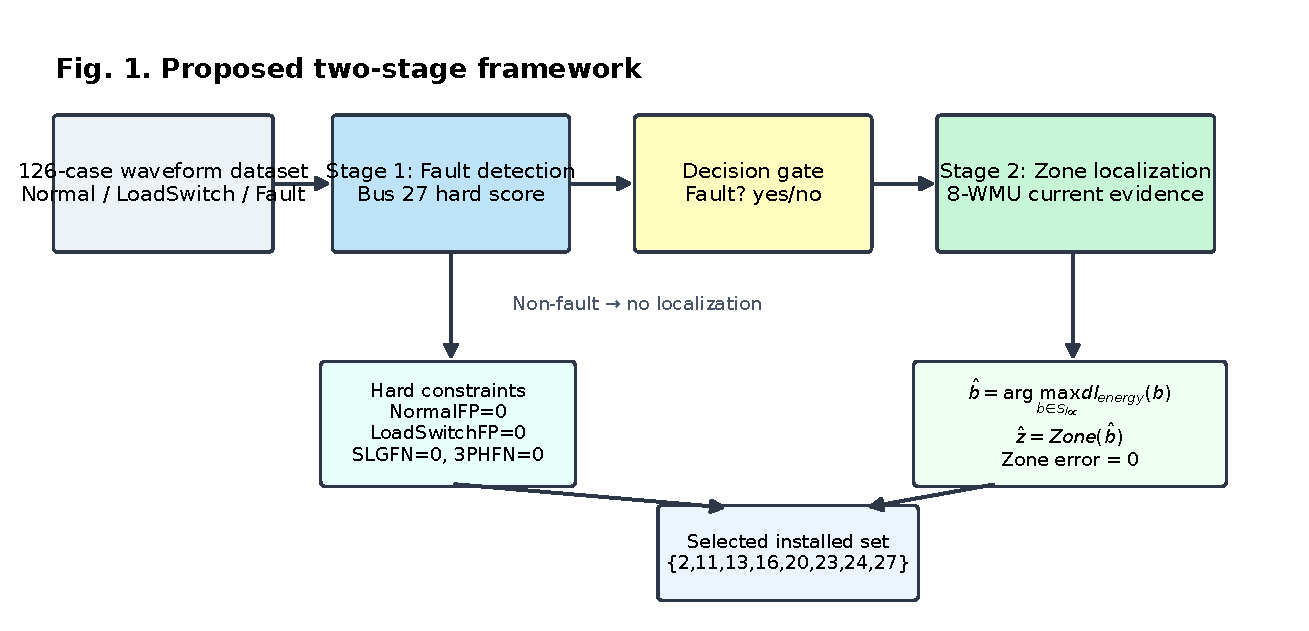
\includegraphics[width=0.95\textwidth]{Fig1_proposed_two_stage_framework.pdf}
\caption{제안하는 two-stage framework. Stage 1은 Bus 27 detection anchor를 이용해 hard-constrained fault detection을 수행하고, Stage 2는 selected eight-WMU localization set을 이용해 current-disturbance 기반 zone localization을 수행한다.}
\label{fig:framework}
\end{figure*}

IEEE 30-bus system의 candidate bus set을 $\mathcal{B}=\{1,2,\ldots,30\}$으로 둔다. 각 event case $i$는 binary label
\begin{equation}
y_i\in\{0,1\}
\end{equation}
을 갖는다. 여기서 $y_i=0$은 normal operation과 LoadSwitch disturbance를 포함하는 non-fault case이고, $y_i=1$은 SLG 및 three-phase fault를 포함하는 fault case이다. Fault case의 실제 faulted bus를 $b_i$로 두면, corresponding topology zone은
\begin{equation}
z_i=Z(b_i)
\end{equation}
이다. 여기서 $Z(\cdot)$는 각 bus를 predefined topology zone으로 mapping하는 함수이다.

Two-stage 구조를 사용하는 이유는 fault/non-fault detection에 충분한 WMU subset과 location identification에 충분한 WMU subset이 서로 다를 수 있기 때문이다. 최종 system은 detection을 위해
\begin{equation}
S_{det}=\{27\}
\end{equation}
을 사용하고, localization을 위해
\begin{equation}
S_{loc}=\{2,11,13,16,20,23,24,27\}
\end{equation}
을 사용한다.

\section{Stage 1: Hard-Constrained Fault Detection}

\subsection{Event Label Definition}

Case $i$의 event type을 $e_i$라고 하자. Non-fault 및 fault event set은 다음과 같이 정의한다.
\begin{equation}
\mathcal{C}_0=\{\mathrm{SSO\_Normal},\mathrm{SSO\_LoadSwitch}\},
\end{equation}
\begin{equation}
\mathcal{C}_1=\{\mathrm{SSO\_SLG\_Fault},\mathrm{SSO\_ThreePhase\_Fault}\}.
\end{equation}
Binary fault label은
\begin{equation}
y_i=\begin{cases}
0, & e_i\in\mathcal{C}_0,\\
1, & e_i\in\mathcal{C}_1.
\end{cases}
\end{equation}
이다. 이 binary mapping은 load switching을 fault가 아닌 normal/non-fault disturbance로 취급하는 protection-oriented transient study의 관점을 따른다.

\subsection{Bus-Wise Normalization and Evidence Features}

Observed bus $b$에서 case $i$의 raw feature value를 $x_{i,b,f}$라고 하자. 각 bus와 feature에 대해 5th 및 95th percentile은 다음과 같이 계산한다.
\begin{equation}
q_{b,f}^{0.05}=Q_{0.05}(\{x_{i,b,f}:i\in\mathcal{I}\}),
\end{equation}
\begin{equation}
q_{b,f}^{0.95}=Q_{0.95}(\{x_{i,b,f}:i\in\mathcal{I}\}).
\end{equation}
Normalized feature는
\begin{equation}
\tilde{x}_{i,b,f}=\mathrm{clip}_{[0,1]}\left(\frac{x_{i,b,f}-q_{b,f}^{0.05}}{\max(q_{b,f}^{0.95}-q_{b,f}^{0.05},\epsilon)}\right),\quad \epsilon=10^{-12}.
\end{equation}
으로 정의한다. 이 normalization은 global이 아니라 observed bus별로 수행하여, 자연적으로 waveform magnitude가 큰 bus가 placement score를 지배하지 않도록 한다.

Fault evidence feature set은 voltage/current disturbance energy, voltage sag, RMS-current jump, sequence/unbalance ratio, apparent-impedance change feature를 포함한다. Compact하게 쓰면
\begin{equation}
\mathcal{F}_{fault}=\{f^{fault}_1,f^{fault}_2,\ldots,f^{fault}_{13}\}.
\end{equation}
LoadSwitch evidence는 three phase의 67--77 Hz voltage cycle-difference ratio에 기반한다.
\begin{align}
\mathcal{F}_{LS}=\{&\mathrm{dV\_E72\_ratio\_A},
\mathrm{dV\_E72\_ratio\_B},\nonumber\\
&\mathrm{dV\_E72\_ratio\_C}\}.
\end{align}

\subsection{Detection Score and Hard Constraints}

각 case와 bus에 대해 fault evidence는
\begin{equation}
F_{i,b}=\max_{f\in\mathcal{F}_{fault}}\tilde{x}_{i,b,f}
\end{equation}
로 정의하고, LoadSwitch evidence는
\begin{equation}
L_{i,b}=\min_{\phi\in\{A,B,C\}}\tilde{x}_{i,b,\mathrm{dV\_E72\_ratio}_{\phi}}
\end{equation}
로 정의한다. Detection anchor $b_d$에 대한 score는
\begin{equation}
s_{i,b_d}=F_{i,b_d}-\lambda L_{i,b_d},\quad \lambda=0.5
\end{equation}
이다. Maximum non-fault score와 minimum fault score는
\begin{equation}
M_0(b_d)=\max_{i:y_i=0}s_{i,b_d},\quad m_1(b_d)=\min_{i:y_i=1}s_{i,b_d}
\end{equation}
이고, separation margin은
\begin{equation}
\gamma_{det}(b_d)=m_1(b_d)-M_0(b_d)
\end{equation}
이다. $\gamma_{det}(b_d)>0$이면 midpoint threshold
\begin{equation}
\tau(b_d)=\frac{M_0(b_d)+m_1(b_d)}{2}
\end{equation}
를 선택한다. Predicted label은
\begin{equation}
\hat{y}_i=\mathbb{I}(s_{i,b_d}>\tau)
\end{equation}
이다.

Detection anchor가 feasible하기 위해서는 다음 hard constraints를 만족해야 한다.
\begin{align}
\mathrm{NormalFP}=0,\quad \mathrm{LoadSwitchFP}=0,\nonumber\\
\mathrm{SLGFN}=0,\quad \mathrm{ThreePhaseFN}=0.
\end{align}
Bus 27은 이 hard constraints를 만족하며 Fig.~\ref{fig:detcm}의 detection confusion matrix를 제공한다.

\begin{figure}[t]
\centering
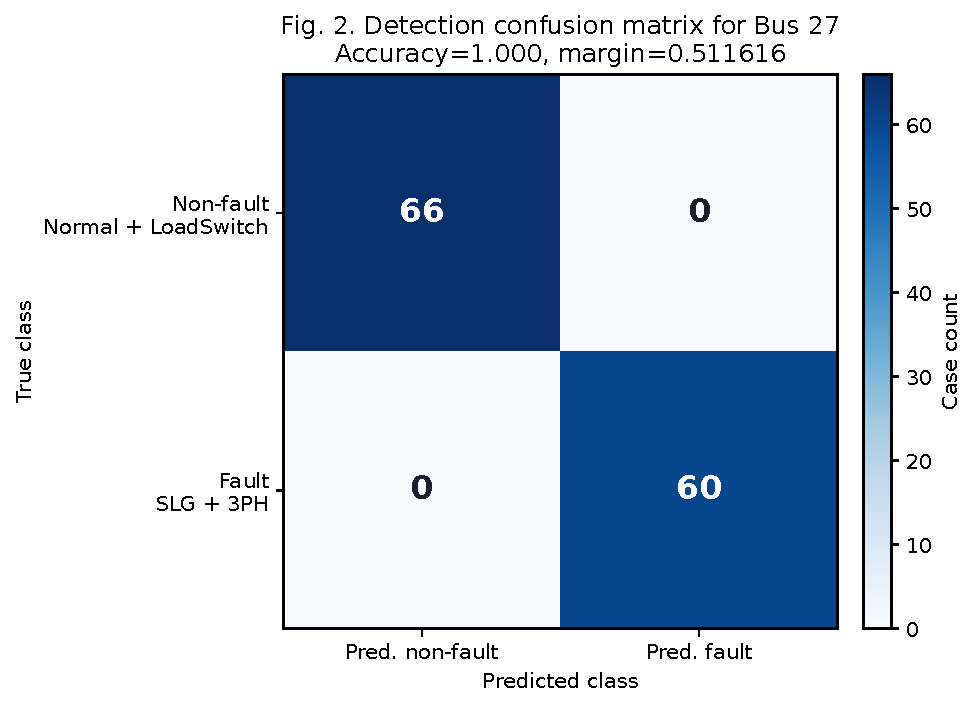
\includegraphics[width=0.95\columnwidth]{Fig2_detection_confusion_matrix_bus27.pdf}
\caption{Bus 27에 대한 detection confusion matrix. 평가 dataset은 66개의 non-fault case와 60개의 fault case를 포함하며, Bus 27은 평가 case에서 zero detection error를 보인다.}
\label{fig:detcm}
\end{figure}

\section{Stage 2: Current-Disturbance-Based Zone Localization}

\subsection{Argmax Localization Rule}

Case가 fault로 분류되면, Stage 2는 faulted topology zone을 추정한다. 각 fault case $i$와 installed localization WMU $b\in S_{loc}$에 대해 localization stage는
\begin{equation}
D_{i,b}=dI\_energy_{3ph,max}(i,b)
\end{equation}
를 사용한다. Predicted location proxy bus는
\begin{equation}
\hat{b}_i(S_{loc})=\argmaxop_{b\in S_{loc}}D_{i,b}
\end{equation}
로 선택하고, predicted fault zone은
\begin{equation}
\hat{z}_i(S_{loc})=Z(\hat{b}_i(S_{loc}))
\end{equation}
이다. 이 rule은 physical interpretability를 갖는다. Current-disturbance energy가 가장 큰 installed WMU를 faulted region의 proxy로 취급하기 때문이다. Fig.~\ref{fig:argmax}는 이 decision rule을 설명한다.

\begin{figure}[t]
\centering
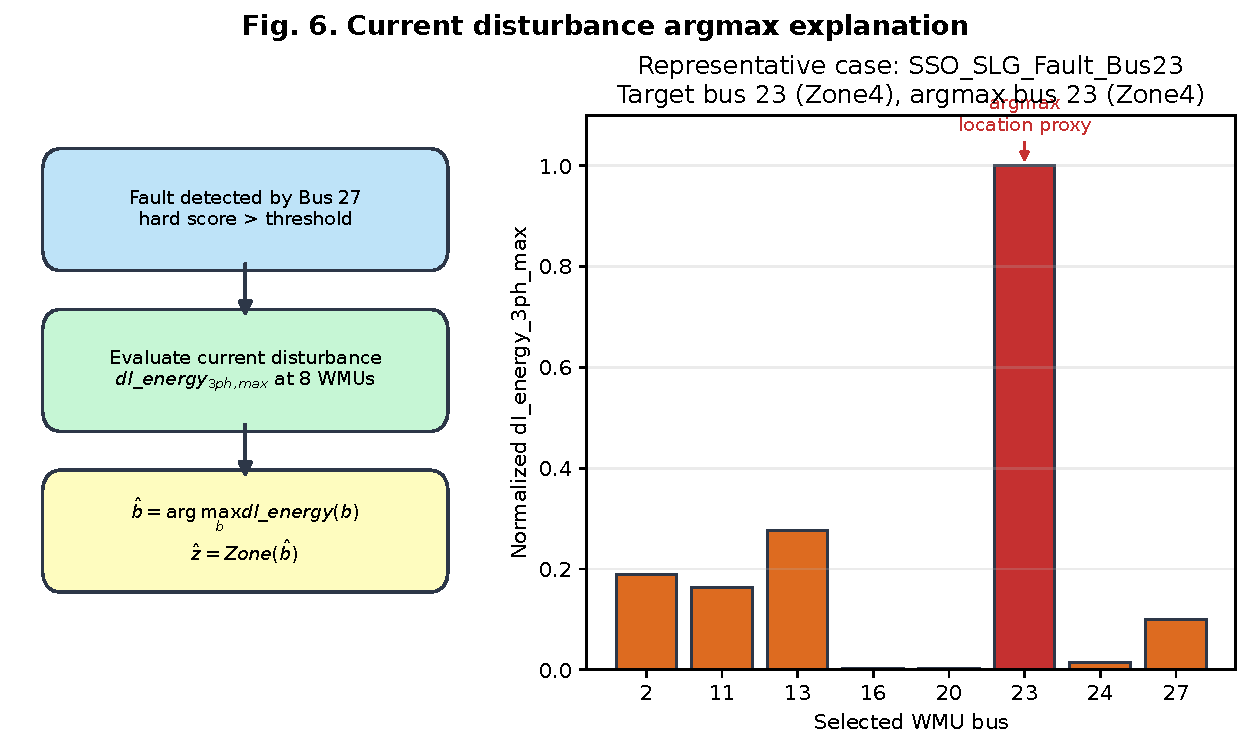
\includegraphics[width=0.98\columnwidth]{Fig6_current_disturbance_argmax_explanation.pdf}
\caption{Current disturbance argmax rule 설명. Fault가 검출되면 localization stage는 selected WMU bus들에서 $dI\_energy_{3ph,max}$를 비교하고, 최댓값을 갖는 bus를 location proxy로 선택한 후 해당 proxy bus를 topology zone으로 mapping한다.}
\label{fig:argmax}
\end{figure}

\subsection{Zone-Localization Constraint}

Localization set $S_{loc}$에 대한 zone-localization error는 evaluated fault-case set $\mathcal{F}$에 대해 다음과 같이 정의한다.
\begin{equation}
\ZoneErr(S_{loc})=\sum_{i\in\mathcal{F}}\mathbb{I}(\hat{z}_i(S_{loc})\neq z_i).
\end{equation}
Localization set은
\begin{equation}
\ZoneErr(S_{loc})=0
\end{equation}
을 만족할 때 feasible하다. Minimum zone-localization placement problem은
\begin{equation}
S^*_{loc}=\argminop_{S\subseteq\mathcal{B}} |S|
\end{equation}
subject to
\begin{equation}
\ZoneErr(S)=0
\end{equation}
로 쓸 수 있다. 따라서 minimum이라는 표현은 지정된 dataset, zone definition, current-disturbance feature, argmax rule에 대한 minimum을 의미한다.

\subsection{Exhaustive Search}

Exhaustive search는 candidate WMU subset의 cardinality를 증가시키면서 모든 subset을 평가한다. 각 subset size $k$에 대해 $|S|=k$를 만족하는 모든 combination $S\subseteq\mathcal{B}$를 test한다. Zero zone error를 만족하는 subset이 처음 등장하는 $k$에서 search를 종료한다. Fig.~\ref{fig:mink}는 search result를 보여준다. $k=1,2,\ldots,7$에서는 zero-error subset이 존재하지 않았고, $k=8$에서 5,852,925개의 evaluated combination 중 5개의 zero-error subset이 발견되었다. 따라서
\begin{equation}
k^*_{zone}=8.
\end{equation}

\begin{figure}[t]
\centering
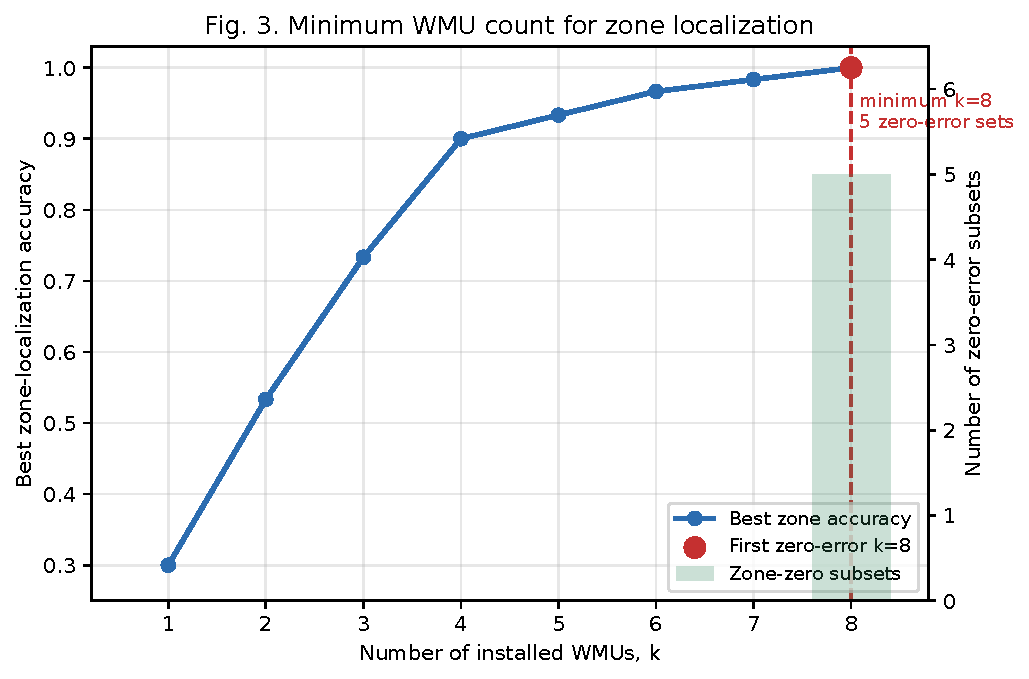
\includegraphics[width=0.98\columnwidth]{Fig3_minimum_wmu_count_zone_localization.pdf}
\caption{Zone localization을 위한 minimum WMU count. Exhaustive subset search 결과 첫 번째 zero-zone-error solution은 $k=8$에서 나타난다.}
\label{fig:mink}
\end{figure}

다섯 개의 feasible eight-WMU subset 중 본 논문은
\begin{equation}
S^*_{loc}=\{2,11,13,16,20,23,24,27\}
\end{equation}
을 선택한다. 이 set은 zero zone-localization constraint를 만족하며 Stage 1에서 식별된 Bus 27 detection anchor를 포함한다. Fig.~\ref{fig:network}는 selected placement를 IEEE 30-bus topology 위에 나타내고, Fig.~\ref{fig:zonecm}는 zone-localization confusion matrix를 보여준다.

\begin{figure}[t]
\centering
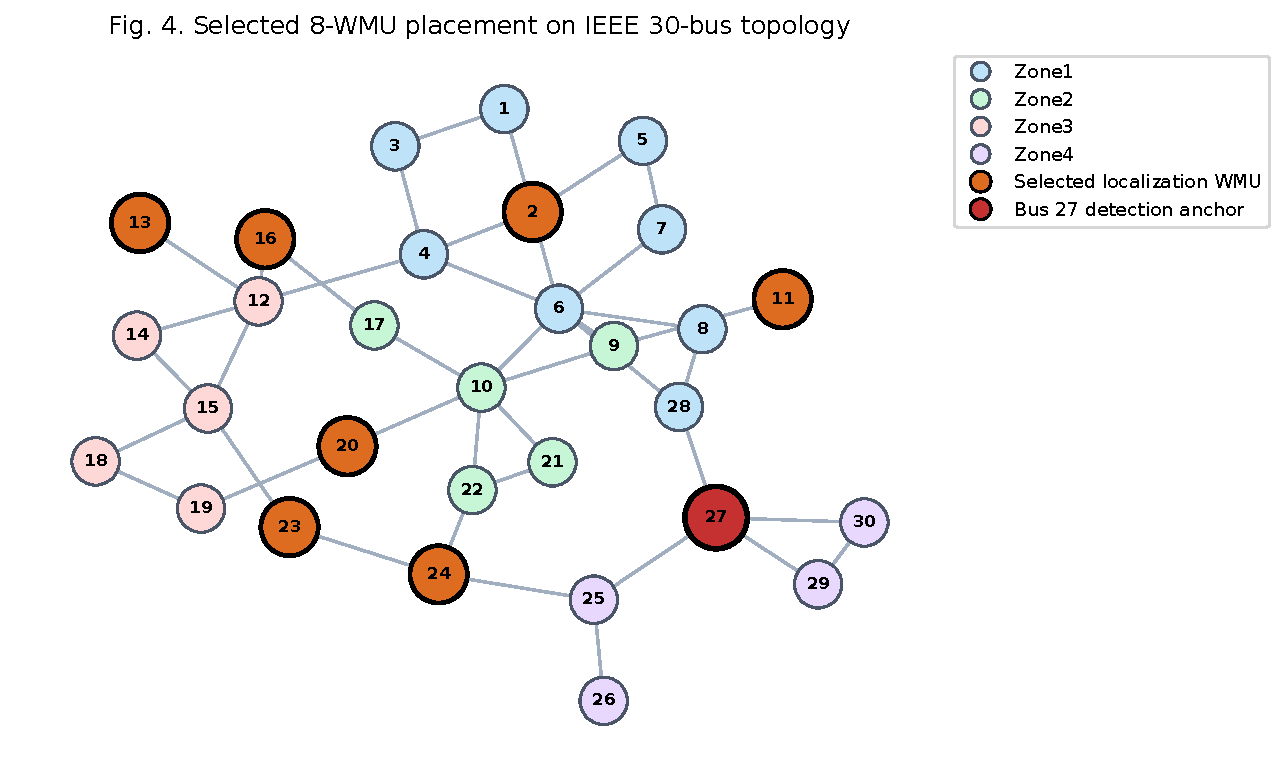
\includegraphics[width=0.98\columnwidth]{Fig4_selected_8wmu_network_map.pdf}
\caption{IEEE 30-bus topology 위의 selected eight-WMU placement. 최종 localization set은 $\{2,11,13,16,20,23,24,27\}$이며, Bus 27은 detection anchor이기도 하다.}
\label{fig:network}
\end{figure}

\begin{figure}[t]
\centering
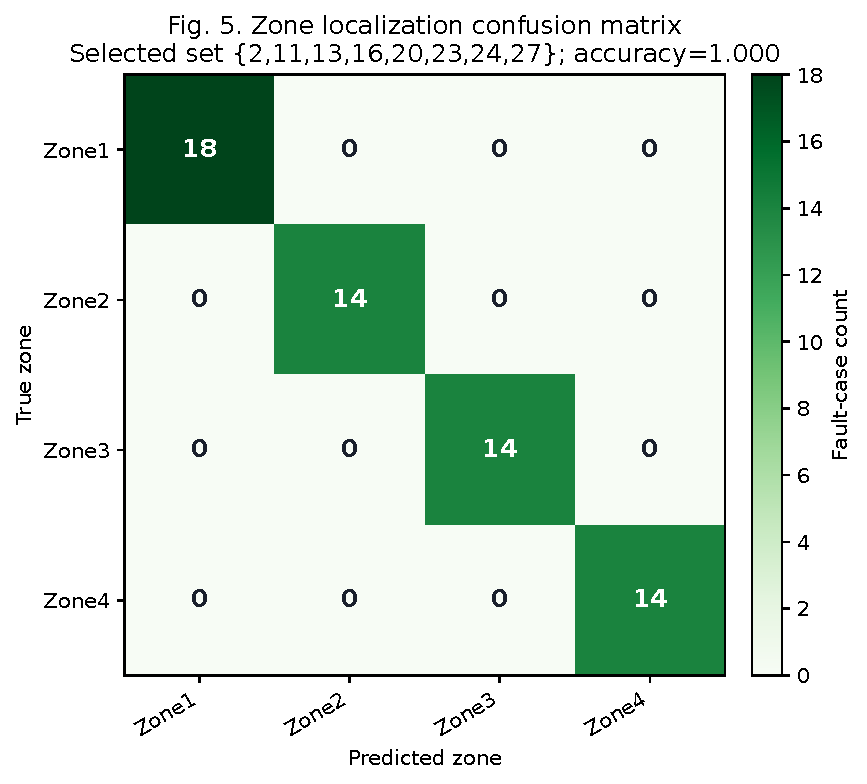
\includegraphics[width=0.95\columnwidth]{Fig5_zone_localization_confusion_matrix.pdf}
\caption{Selected eight-WMU set의 zone localization confusion matrix. Selected placement는 60개의 evaluated fault case 전체에서 zero zone-localization error를 달성한다.}
\label{fig:zonecm}
\end{figure}

\section{Case Study}

\subsection{Test System and Dataset}

Case study는 modified IEEE 30-bus system을 사용한다. Weak-grid IBR interaction과 관련된 oscillatory monitoring condition을 반영하기 위해 모든 event class에 IBR-like 25 Hz SSO background를 포함하였다. Dataset은 Table~\ref{tab:dataset}에 요약한 126개의 deterministic simulation case로 구성된다.

\begin{table}[t]
\caption{Combined Dataset Composition}
\label{tab:dataset}
\centering
\begin{tabular}{llcc}
\toprule
Event type & Magnitude & Cases & Binary class\\
\midrule
SSO\_Normal & -- & 3 & Non-fault\\
SSO\_LoadSwitch & 5\% & 21 & Non-fault\\
SSO\_LoadSwitch & 15\% & 21 & Non-fault\\
SSO\_LoadSwitch & 30\% & 21 & Non-fault\\
SSO\_SLG\_Fault & -- & 30 & Fault\\
SSO\_ThreePhase\_Fault & -- & 30 & Fault\\
\midrule
Total & -- & 126 & --\\
\bottomrule
\end{tabular}
\end{table}

Dataset은 66개의 non-fault case와 60개의 fault case를 포함한다. LoadSwitch case는 5\%, 15\%, 30\% magnitude로 나누어, selected placement가 non-fault switching severity 변화에도 feasible한지 평가한다.

\subsection{Detection Result}

Bus 27 detection anchor는 평가 case에서 false positive와 false negative를 모두 0으로 만든다. Table~\ref{tab:bus27}은 결과를 요약한다. Score separation은
\begin{equation}
-0.038596 < 0.217212 < 0.473020
\end{equation}
을 만족한다. 여기서 $-0.038596$은 largest non-fault score, $0.473020$은 smallest fault score, $0.217212$는 threshold이다. Margin은 $0.511616$이다.

\begin{table}[t]
\caption{Selected Bus 27 Detection Performance}
\label{tab:bus27}
\centering
\begin{tabular}{lc}
\toprule
Metric & Value\\
\midrule
Selected detection WMU & Bus 27\\
NormalFP & 0\\
LoadSwitchFP & 0\\
SLGFN & 0\\
ThreePhaseFN & 0\\
TotalFP / TotalFN & 0 / 0\\
Binary accuracy & 1.000\\
Non-fault max score & -0.038596\\
Fault min score & 0.473020\\
Threshold & 0.217212\\
Fault-score margin & 0.511616\\
\bottomrule
\end{tabular}
\end{table}

\subsection{Localization Result}

Localization exhaustive search result는 Table~\ref{tab:locsearch}에 요약한다. Best zone accuracy는 $k$가 증가할수록 향상되지만, zero-zone-error subset은 $k=8$ 이전에는 존재하지 않는다.

\begin{table}[t]
\caption{Exhaustive Zone-Localization Search Summary}
\label{tab:locsearch}
\centering
\begin{tabular}{cccc}
\toprule
$k$ & Total subsets & Zero-error subsets & Best accuracy\\
\midrule
1 & 30 & 0 & 0.5000\\
2 & 435 & 0 & 0.7167\\
3 & 4,060 & 0 & 0.8333\\
4 & 27,405 & 0 & 0.9000\\
5 & 142,506 & 0 & 0.9500\\
6 & 593,775 & 0 & 0.9667\\
7 & 2,035,800 & 0 & 0.9833\\
8 & 5,852,925 & 5 & 1.0000\\
\bottomrule
\end{tabular}
\end{table}

Selected localization set $\{2,11,13,16,20,23,24,27\}$은 모든 evaluated fault case에 대해 zero zone-localization error를 달성한다. 이 set이 Bus 27 detection anchor를 포함하므로, 최종 two-stage installation은 localization placement 외부에 별도의 detection-only sensor를 요구하지 않는다.

\section{Discussion}

제안 결과는 fault detection과 fault localization의 차이를 분명히 보여준다. 평가한 hard constraints 하에서 Bus 27 단일 WMU는 binary fault detection에 충분하다. 그러나 검출된 fault를 올바른 topology zone으로 localize하려면 더 큰 sensor set이 필요하다. Exhaustive search 결과, 지정된 feature, zone definition, argmax rule 하에서는 $k\leq 7$인 어떤 subset도 zero zone error를 만족하지 못하며, 첫 feasible localization solution은 $k=8$에서 나타난다.

이 차이는 detection-only result의 과도한 해석을 방지한다. 단일 WMU가 평가 dataset에서 fault/non-fault case를 분리할 수 있다는 이유만으로 모든 monitoring objective를 해결한다고 주장해서는 안 된다. 대신 제안하는 two-stage architecture는 fault-zone identification을 지원하기 위해 필요한 추가 WMU requirement를 명시적으로 정량화한다.

또한 본 결과는 주의해서 해석해야 한다. Dataset은 deterministic이며 operating-condition diversity가 제한적이다. Normal case 수가 제한적이고, stochastic load variation은 포함되어 있지 않으며, SSO background도 고정되어 있다. Measurement noise, missing channel, communication delay, synchronization error, fault resistance variation, inception-angle variation 등은 향후 validation에 포함되어야 한다.

\section{Conclusion}

본 논문은 IBR-like oscillatory background condition 하에서 fault detection과 zone localization을 위한 two-stage hard-constrained WMU placement framework를 제안하였다. Stage 1은 Bus 27을 detection anchor로 사용하며, 평가 dataset에서 NormalFP, LoadSwitchFP, SLGFN, ThreePhaseFN을 모두 0으로 만들고 fault-score margin 0.511616을 달성한다. Stage 2는 installed WMU set에 대해 current-disturbance-based argmax rule을 사용하여 localization을 수행한다. Exhaustive search 결과, zero-error zone localization은 $k=8$에서 처음 feasible해지며, selected final placement는 $\{2,11,13,16,20,23,24,27\}$이다. 본 연구는 minimum WMU requirement가 monitoring objective에 따라 달라짐을 보여준다. 평가한 detection task에는 1개의 WMU가 충분하지만, 지정된 formulation 하에서 zero-error zone localization을 달성하려면 8개의 WMU가 필요하다.

향후 연구에서는 SSO frequency, SSO amplitude, damping, load level, fault resistance, fault inception angle, measurement noise, missing data, synchronization error 등을 변화시켜 dataset을 확장해야 한다. 또한 hard-constrained framework는 train/validation/test thresholding, N-1 sensor contingency constraint, joint detection--classification--localization placement로 확장될 수 있다.

\bibliographystyle{IEEEtran}
\bibliography{references}

\end{document}
